% !Tex root = ../main.tex

\chapter{在隐私保护上的应用}\label{chp:application}

% 在这一章,我们主要调研了近年来发表在安全顶会上的论文,

这一章我们主要介绍布隆过滤器及其衍生数据结构在隐私保护相关协议中的应用。
其中涉及到的协议包括可搜索加密、隐私信息检索和隐私集合运算。
% 其中
% 本章涉及到的协议包括可搜索加密、隐私信息检索和隐私集合运算。
% 我们挑选了近年来
% 我们挑选了近年来发表在顶会上的论文,通过
% 可搜索加密、隐私信息检索和隐私集合计算三个密码学协议,并结合近年来发表的工作

\section{在对称可搜索加密方面的应用}

\subsection{背景介绍}

% 可搜索加密的定义,分类,系统模型
% 可搜索加密(searchable encryption)针对的外包加密文件上的搜索问题。
随着近年来数据规模的不断增大,越来越多的个人和企业选择将本地文件外包到云平台(如 iCloud、Amazon S3)进行存储。
% 数字化程度不断提高,文件
存储在云端的文件不仅为用户节省了本地存储所需要的成本,避免文件丢失的风险,还能让用户随时随地通过互联网对文件进行搜索和访问,极大地提高了便利性。
但是将文件直接存放在云服务器中也大大增加文件泄露的风险。
% 对于服务器内部来说,云服务提供商可以直接获取存储的文件;而
一方面云服务提供者可以直接获取文件,另一方面由于云服务器处在公开的网络环境中,很容易受到外部攻击者的攻击。
一旦文件遭到泄露,用户的隐私也受到威胁。
保护用户文件隐私的直接方式是将文件在本地进行加密,再将加密后的文件进行上传。
但是服务器无法在加密后的文件上执行搜索,用户需要搜索时只能把所有文件下载下来才能完成,这就丧失了将文件存储在云端的意义。
% 上传之前对文件加密,
% 但是这样一来服务器便无法对数据进行搜索,丧失了

为了解决文件隐私和可搜索之间的矛盾,对称可搜索加密(Searchable Symmetric Encryption,SSE)~\cite{song2000practical,curtmola2006searchable}的概念被提出。
对称可搜索加密通过为加密数据构造安全索引实现隐私保护的关键词搜索。
如图所示,对称可搜索加密中包含用户和服务器两个实体。
在上传阶段,用户不仅需要上传加密文件,还需要上传对应的安全索引。
在搜索阶段,用户根据需要搜索的关键词生成搜索 tokens,服务器使用搜索tokens检索得到加密的文件标识并返回给用户。

% 从对称可搜索加密的搜索过程可以看出,
我们假设服务器是半诚实的(semi-honest),即服务器会诚实地执行协议,但它同时会对尝试分析输入输出信息来推断用户的隐私。
相比其他隐私保护的搜索方案,对称可搜索加密方案能在效率和安全之间取得更好的平衡。
% 在效率和安全之间
一方面,基于属性保留加密(Property-Preserving Encryption)的方案~\cite{bellare2007deterministica}可以直接保留密文中的相等关系,从而实现高效的搜索。
但服务器可以通过分析密文上的相等信息来执行频率统计攻击并还原明文信息~\cite{naveed2015inferencea}。
在另一方面,基于通用密码学工具(如同态加密、安全多方计算以及不经意随机访问机)虽然能够提供较强的安全性,但这些工具要么在计算上开销非常大,要么存在较大的通信开销,直接应用到加密搜索场景会面临效率问题~\cite{ren2023searchable}。
% 同态加密或多方安全计算虽然能够提供较强的安全性,但同态加密方案需要
而对称可搜索加密通过将搜索过程转移到安全索引上,在允许有限信息泄露的同时提供了高效的搜索。

目前安全索引大多以倒排索引形式构建,也就是利用关键词信息去匹配文件标识的形式。
这样能够保证搜索效率只与关键词对应的文件数有关,而与整个数据库的大小无关。
对称可搜索加密允许泄露的信息也被称作模式信息(pattern information),这些信息包括:
\begin{itemize}
  \item 搜索模式(search pattern),即两次搜索是否包含相同的搜索关键词。
  \item 访问模式(access pattern),即每次搜索能匹配到哪些加密结果。
  \item 数量模式(volume pattern),即每次搜索返回的结果数量。
\end{itemize}
% 允许泄露这些信息是为了
对称可搜索加密协议的安全性是定义在给定的模式信息之上的,也就是说如果我们称一个对称可搜索加密协议是安全的,那么除了允许泄露的模式信息之外,它不会泄露其他的任何信息。
% 所以说对称可搜索加密方案是牺牲一定的安全性来换取搜索效率。
近些年有大量工作~\cite{cash2015leakageabuse,grubbs2018pump,gui2019encrypted,blackstone2020revisiting,ning2021leap,kamara2022sok}集中关注于如何利用这些模式信息来设计相应的攻击,这些攻击被统称为泄露滥用攻击(Leakage-Abuse Attacks, LAAs)。
而我们前面的介绍的过滤器及其衍生数据结构正好可以用来隐藏特定的模式信息,从而避免受到对应的攻击。
以下我们将给出两个具体例子,介绍这些数据结构是如何用到对称可搜索加密之中的。

% 索引形式,倒排索引

\subsection{HXT}

这一节我们介绍的是 HXT (Hidden Cross-Tags) 协议~\cite{lai2018result}。
HXT 是一个针对连接多关键词查询的可搜索加密协议。
上一节介绍的内容都是默认只考虑单关键词查询,如果要扩展到多关键词并不是一件容易的事。
最直接的方式是执行多次单关键词的查询,但这样做,一来服务器与用户之间交互次数太多,通信开销太大;二来服务器可以知道每次查询的各种模式信息。
针对这些问题,Cash等人提出了次线性(sublinear)的连接多关键词协议 OXT (Oblivious Cross-Tags),即对于任意形如 $w_1\land w_2 \land \dots \land w_n$ 的连接多关键词查询,OXT 的查询复杂度只与第一个关键词对应的文件数量有关(次线性),与查询的关键词数量、数据库中文件数量无关。
OXT 协议中包含两个索引,分别为 T-set 和 X-set,其中 T-set 与倒排索引类似,X-set 则是存储每个关键词 $w$ 与文件标识 $ind$ 配对的加密形式(称为 xtag)。
% 元组,如 $(w, ind)$ 形式。
% 通过构造两个索引
搜索时,用户首先选取搜索关键词中对应预估文件数最低的关键词(称为 s-term)生成对应在 T-set 中的搜索token(称为 stag),并生成其他搜索关键词(称为 x-term)对应的搜索tokens(称为 xtokens)。
以形如 $w_1 \land w_2 \land \dots \land w_n$ 的连接多关键词为例,其中假设 s-term 为 $w_1$。
服务器在收到这些搜索tokens之后,首先根据 stag 从 T-set 中检索出 $w_1$ 对应的加密文件标识列表和盲化的关键词与文件标识配对列表。
然后在上一步检索结果的基础上,使用 xtokens 还原出对应的 xtag,如果该 xtag 存在于 X-set 中,则返回对应的加密文件标识。
% 再利用 xotkens
% 与这些盲化的关键词与文件标识配对
图~\ref{fig:oxt_example}~对OXT协议的搜索过程进行了描述。
从整体上来看,OXT 协议的核心思路是先通过 T-set 确定出一个较小的文件范围,再使用 X-set 从这些文件中筛选出符合条件的结果。
这样就避免了前面提到的交互次数太多和泄露每个单独关键词模式信息的问题,而且能够实现次线性的搜索复杂度。
% 就能将搜索复杂度限制为 s-term 对应的文件数量。
但是在 OXT 协议中,因为需要计算出每个 x-term 与 s-term 对应的文件标识配对的 xtag,而服务器可以判断每一个 xtag 是否存在于 XSet 中。
以图~\ref{fig:oxt_example}~中的查询为例,服务器可以判断关键词 $w_2$ 与 $ind_1$ 配对的 xtag 存在于 X-set,而关键词 $w_3$ 与 $ind_1$ 配对的 xtag 不存在于 X-set。
Lai 等人~\cite{lai2018result} 将这种信息定义为关键词对结果模式 (Keyword Pair Result Pattern, KPRP)。
而 HXT 协议的提出就是为了解决 OXT 中 KPRP 信息泄露问题。
% 为了防止 KPRP 的信息泄露,
% OXT 协议的
\begin{figure}[ht]
  \centering
  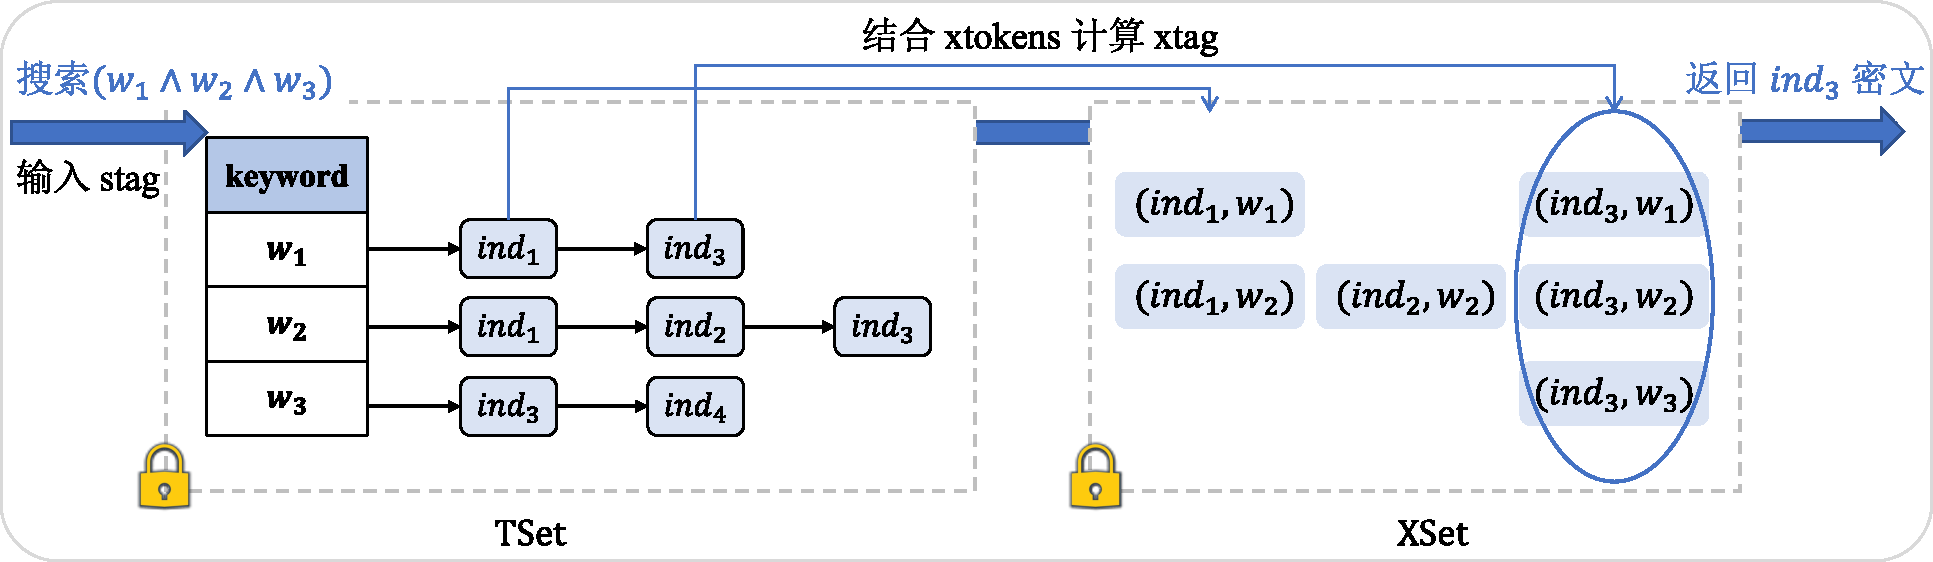
\includegraphics[width=\textwidth]{figures/OXT_exp.pdf}
  \caption{OXT 协议查询流程示例}
  \label{fig:oxt_example}
\end{figure}

HXT 协议相比 OXT 协议主要修改的是 X-set 构造。
为了隐藏 KPRP,就需要保证服务器不能通过计算 xtag 来完成在 X-set 中的筛选,也就是说 X-set 中不能直接保存 xtag。
% 因此在 HXT 协议中,
HXT 协议采用的方法是将 X-set 使用布隆过滤器构造成长度为 $m$ 的数组,再通过对称隐藏向量加密 (Symmetric Hidden Vector Encryption, SHVE) 进行加密,将加密结果作为 HXT 中的 X-set,如图~\ref{fig:xset_example}~所示。
\begin{figure}[ht]
  \centering
  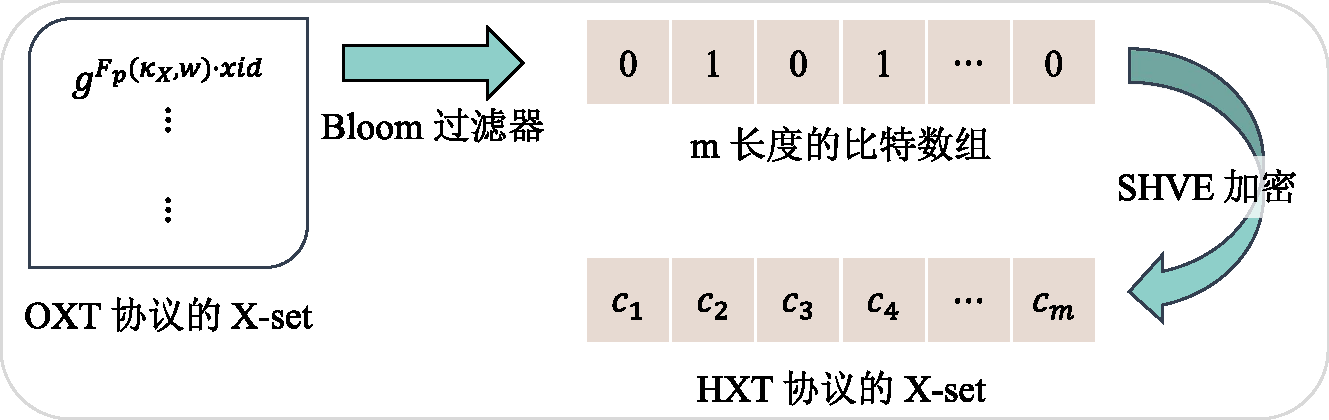
\includegraphics[width=0.95\textwidth]{figures/xset_exp.pdf}
  \caption{HXT 协议中 X-set 的构造}
  \label{fig:xset_example}
\end{figure}

SHVE 是一种针对 $0/1$ 比特向量的加密算法,它主要包含以下四个算法:
% 特点是当查询向量能够与加密的向量成功匹配时,SHVE
\begin{itemize}
  \item $\mathsf{SHVE}.\mathsf{Setup}(\lambda) \to msk$:通过输入安全参数 $\lambda$,输出主密钥 $msk$,并定义明文空间 $\mathcal{M}$。
  \item $\mathsf{SHVE}.\mathsf{KeyGen}(msk, \mathbf{v} \in \{0,1,*\}^m \to \mathbf{s} $:通过输入长度为 $m$ 的预测向量 $\mathbf{v}$ 和主密钥,输出解密密钥 $\mathbf{s}$。
  \item $\mathsf{SHVE}.\mathsf{Enc}(msk, \mu\in \mathcal{M}, \mathbf{x} \in \{0,1\}^m ) \to \mathbf{c}$:通过输入明文消息 $\mu$ 和长度为 $m$ 的索引向量 $\mathbf{x}$,输出密文 $\mathbf{c}$。
  \item $\mathsf{SHVE}.\mathsf{Query}(\mathbf{s}, \mathbf{c}) \to \mu \mbox{ or} \perp$:通过输入预测向量 $\mathbf{v}$ 对应的解密密钥 $\mathbf{s}$ 和密文 $\mathbf{c}$,如果$P_{\mathbf{v}}^{\mathsf{SHVE}}(\mathbf{x}) = 1$,则返回明文消息 $\mu$;否则返回 $\perp$。
\end{itemize}
其中 $P_{\mathbf{v}}^{\mathsf{SHVE}}(\mathbf{x})=1$ 的含义是向量 $\mathbf{v}$ 和 $\mathbf{x}$ 除了通配符 $*$ 所在位置上,其他所有位置上的值都相等,即
\begin{equation}
  P_{\mathbf{v}}^{\mathsf{SHVE}}(\mathbf{x}) = \left\{
  \begin{array}{ll}
  1 & \forall 1\leq i \leq m \  (v_i = x_i \mbox{ or } v_i=*), \\
  0 & \mbox{otherwise}. \\
  \end{array}
  \right.
\end{equation}
关于方案的具体构造可以参考文献~\cite{lai2018result},这里就不详细介绍。
% 这里我们不介绍
这里主要介绍 HXT 是如何结合 SHVE 来隐藏 KPRP 的。
构造时,用户使用图~\ref{fig:xset_example}~中的方式构造 X-set,在使用 SHVE 加密时,明文消息 $\mu$ 设置为 True。
% 在生成 stag 和 xtoken 部分,HXT 与 OXT 类似。
搜索时,用户还是首先生成 stag 和 xtoken,这部分 HXT 与 OXT 相同。
服务器还是通过 stag 检索 T-set,再利用 xtoken 计算出一系列 xtag。
% 在服务器收到
由于此时 X-set 中并没有直接存储 xtag,所以服务器并不能直接通过 xtag 完成判断。
% 与布隆过滤器的
对于服务器使用 stag 检索出的每个加密文件标识,后续的判断过程如下:
\begin{itemize}
  \item 服务器使用布隆过滤器的哈希函数,计算 xtag 对应的位置,并返回给用户。
  \item 用户生成长度为 $m$ 且所有位置为 $*$ 的向量 $\mathbf{v}$,根据服务器返回的位置,将向量 $\mathbf{v}$ 上所有这些位置上的值设为 $1$。
  \item 用户调用 $\mathsf{SHVE}.\mathsf{KeyGen}$ 将生成向量 $\mathbf{v}$ 对应的解密密钥并发送给服务器。
  \item 服务器调用 $\mathsf{SHVE}.\mathsf{Query}$ 来判断 $\mathbf{v}$ 是否能与 X-set 匹配,如果返回为 True,则将对应的加密文件标识返回给用户。
\end{itemize}
相比于 OXT 协议,HXT 在搜索时需要多一轮通信,目的是让用户生成判断向量 $\mathbf{v}$。
%
% 从上述搜索过程可以看出,
得益于布隆过滤器的特性,向量 $\mathbf{v}$ 记录了所有 x-term 的信息,服务器只能判断每个加密文件标识是否满足查询条件中的 x-term,并不能判断每个单独的 x-term 与加密文件标识的对应关系,从而避免 KPRP 信息的泄露。
% 服务器只能判断每个加密文件标识是否满足查询条件,从而避免
% 对于服务器而言,

% 在 HXT 协议中,X-set 不再存储
% HXT~\cite{lai2018result}
% 本节我们介绍的协议

\subsection{XorMM}

这一节介绍的 XorMM~\cite{wang2022practical}是一个借助异或过滤器隐藏数量模式的对称可搜索加密协议。
数量模式指的是在搜索过程中,服务器获取的查询结果数量信息。
% 在早期的可搜索加密中,
早期的可搜索加密方案中认为这类模式信息的泄露是可以接受的。
但近年来的研究~\cite{grubbs2018pump,gui2019encrypted,blackstone2020revisiting}指出,攻击者可以利用数量模式推测用户搜索的关键词甚至还原出用户存储的信息。
因此隐藏数量模式就显得尤为重要。

要隐藏数量模式,最直接的思路是采用填充的方式,将倒排索引中每个关键词对应的文件数量填充为相同的长度。
% 每次搜索强制让服务器返回相同数量的结果。
% 因此服务器就需要存储
这样无论是搜索哪个关键词,服务器查找得到的结果数量都相同,从而隐藏了每个关键词实际对应的数量模式信息。
现有工作~\cite{ando2022cost}认为,要实现隐藏数量模式信息的目的,填充后每个关键词对应的结果数量至少为填充前结果数量的最大值。
% 但是直接填充的话
这也就意味着填充后索引的存储开销会非常大,在实际中不可行。

为了解决这一问题,XorMM~\cite{wang2022practical}提出将异或过滤器的结构作为可搜索加密中的索引。
% 我们暂时不考虑对关键词和文件标识的加密,
以关键词 $w_1$ 对应文件标识 $\{ind_1, ind_2, ind_3\}$ 为例,XorMM 中将其看作 $\{(w_1 ||1, ind_1), (w_1 || 2, ind_2), (w_1 || 3, ind_3)\}$ 这样的键值型组合集合。
这样一来便可以使用异或过滤器对其进行记录,比如将 $ind_1$ 看作 $w_1 || 1$ 对应的指纹,查询时只需要输入 $w_1 || 1$,则返回对应的 $ind_1$。
而对于不存在的键,比如 $w_1||4$,还是能够得到其对应的结果。
% 为了确保
以上描述的是明文索引的构造思路,对于安全索引,我们只需要将所有的关键词替换成对应的关键词 token,而文件标识也需要替换成对应的密文形式。
这样构造的安全索引就能在不需要填充的情况下实现对任意查询都能返回一个确定的结果。
% 在构造索引之前,需要将

% 尽管采用异或过滤器
按照上述方式构造的安全索引能够实现较低的存储开销,但用户在查询时还存在通信开销上的问题。
假设 $\ell$ 为数量模式的最大值,为了隐藏数量模式,就需要每次搜索时让服务器都返回 $\ell$ 个搜索结果。
以查询关键词 $w_1$ 为例,用户需要发送 $\{w_1 || 1, w_1 ||2, \dots, w_1 || \ell \}$ 对应的搜索 tokens,这会造成非常大的通信开销。
为了解决这个问题,XorMM 采用受限伪随机函数(Constrained Pseudorandom Function, CPRF)让服务器可以根据用户给定的密钥独自生成 $\ell$ 个搜索 tokens,从而避免通信开销问题。
图~\ref{fig:xormm_example}~给出了XorMM协议的查询流程。
主要分为以下几个步骤:
\begin{itemize}
  \item 用户根据查询关键词生成对应的 CPRF 密钥 $tk_{key}$,以及设定的返回结果数量 $\ell$,并发送给服务器。
  \item 服务器根据 $tk_{key}$ 生成 $\ell$ 查询关键词对应的 $\ell$ 个搜索 tokens,并通过异或过滤器得到 $\ell$ 个对应的结果,最后将结果放回给用户。
\end{itemize}
\begin{figure}[ht]
  \centering
  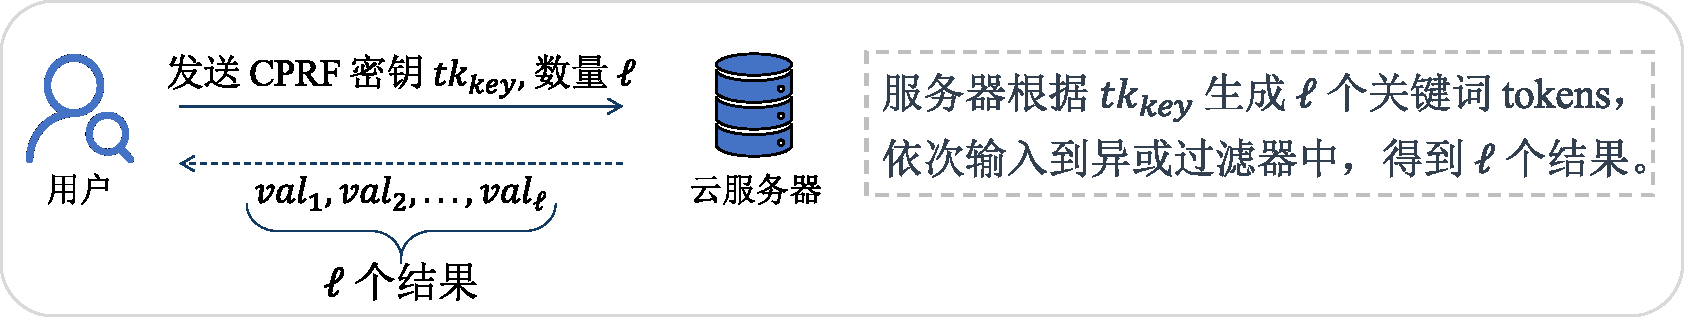
\includegraphics[width=\textwidth]{figures/xormm_exp.pdf}
  \caption{XorMM 协议查询示例}
  \label{fig:xormm_example}
\end{figure}
在XorMM的协议设计中,我们可以发现异或过滤器的作用更像是不经意随机键值存储。
正如我们在

\section{在隐私信息检索方面的应用}

\subsection{背景介绍}


\subsection{方案介绍}

\section{在隐私集合运算方面的应用}

\subsection{背景介绍}

% \subsection{方案介绍}
\subsection{隐私集合求交的协议}

\subsection{隐私集合求并的协议}

\section{总结}
